\chapter{Introducción}

\section{ Motivación y objetivos}

Durante el desarrollo humano, las células están expuestas a una compleja red de señales reguladoras las cuales deben interpretar correctamente para desarrollar las funcionalidades necesarias requeridas por el organismo. Por tanto, se pueden entender la transducción de señales y las cascadas de regulación genética como mecanismos de procesamiento de la información que traducen la información extracelular en decisiones intracelulares.

El presente trabajo pretende mostrar las diferencias en cuanto a comportamiento cualitativo que se pueden encontrar modelando estos complejos sistemas de regulación biológicos mediante distintas aproximaciones teóricas. 

En particular, nos centraremos en el estudio del sistema de señalización del Sonic Hedgehog (en adelante Shh). 
El Shh es una proteína que conforma uno de los factores de señalización  canónicos, secretados
para regular la función celular y, por tanto, el desarrollo en numerosos sistemas.
\begin{figure}[h]
	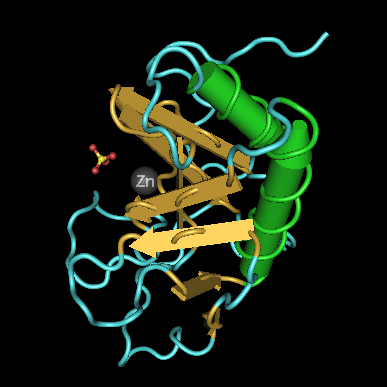
\includegraphics[width=0.5\textwidth]{shh_protein}
	\centering
	\caption{Representación esquemática de la proteina de Shh. Fuente: \cite{wiki:foto_shh}}
\end{figure}


Por ejemplo, la importancia del Shh se pone de manifiesto teniendo en cuenta algunos de sus muchos roles durante el desarrollo: 
\begin{itemize}
	\item Modela la diferenciación del tejido de la médula espinal.
	\item Modela la diferenciación del tejido de la la yema del miembro.
	\item Controla la diferenciación neuronal del mesencéfalo. 
	\item Controla la diferenciación neuronal del prosencéfalo ventral.
\end{itemize}

Una de las características más importantes es que el Shh puede modelar distintos tejidos durante el desarrollo formando un gradiente de concentración \cite{saha}. Debido a este gradiente las células detectan su posición dentro del mismo y se diferencian en distintos fenotipos \footnote{Denominamos fenotipo a la expresión del genotipo, es decir, la expresión de los genes, en función de un determinado ambiente.} según la concentración y el tiempo de exposición a la concentración.

Aparte, como se destaca en \cite{schaffer} el Shh también
controla la proliferación de numerosas poblaciones de células durante el desarrollo, incluidas las células granulares del cerebelo. Esto implica que las mutaciones dentro del sistema de señalización/regulación del Shh se han asociado con la proliferación de tumores (cáncer) en numerosos tejidos, como en el reciente articulo \cite{clement2007hedgehog}.

Con esta breve introducción ponemos de manifiesto la importancia de conocer el comportamiento de estas redes de señalización. Nuestro interés principal será conocer como afecta de manera cualitativa, un cambio en el procedimiento teórico de modelado de los mecanismo bioquímicos involucrados en la expresión genéticas. Centrándonos en redes de regulación/expresión que relacionan las proteínas\textit{ Ptc, Gli} y \textit{Shh.}

Acotando aún más el sujeto de estudio, los factores de transcripción dentro de la familia \textit{Gli} desempeñan papeles críticos en la mediación e interpretación de las señales de Shh \cite{i1999proteins}. Elucidar cómo funcionan nuestras redes de regulación y las proteínas \textit{Gli} nos permitirá ampliar nuestro conocimiento de cómo las células proliferan, diferencian o sobreviven en respuesta a señales de \textit{Shh}, procesos con importancia capital en una gran cantidad de aspectos como por ejemplo \cite{dahmane1997activation}. En especial es importante conocer de qué manera afectan estos cambios a la aparición/desaparición y/o existencia/inexistencia de estados estables o metaestables. Y, por supuesto, de como están relacionados y como podemos llegar de unos a otros. 
 
 Nuestro trabajo recoge un estudio completo del modelo clásico propuesto en \cite{schaffer}, aportando nueva información dentro del mismo, y un conjunto de experimentos numéricos relacionando nuevos desarrollos teóricos con el modelo clásico. 
 
 Además, al contrario que los artículos originales, todos los códigos se encuentran online y libres para su uso y reproducibilidad, vía archivos y vía \textit{Jupyter Notebooks}.
 
 Por otra parte, presentamos un estudio teórico y numérico de una nueva forma de modelar desde el enfoque termodinámico este proceso, propuesta en \cite{multiple} para comparar las diferencias cualitativas entre ambos, y avanzar qué posibles resultados podríamos obtener de este nuevo modelo. 
 
 \section{Sistema de señalización de Shh}
 
 En esta sección pretendemos ofrecer una visión general de la red de regulación de Shh que se observa en la célula. Todos los modelos usados dentro de este trabajo poseen puntos de vista compartidos, por lo que todas aquellas características que comparten ambos modelos se pueden encontrar aquí.
 
 Asi pues, se puede encontrar en esta sección la descripción bioquímica del sistema de señalización de Shh y las ecuaciones estándar empleadas en los procesos e interacciones bioquímicas que poseen ambos modelos.
 
 \subsection{Descripción bioquímica del proceso}
 
 La red de señalización de \textit{Shh} comprende la actividad de varias proteínas \ref{figuras} y genes :
 \begin{itemize}
 	\item \textbf{Sonic Hedgehog (Shh)}. Gen: \textit{shh}\footnote{ De forma convencional los genes que codifican una determinada proteína vienen expresados con el mismo nombre, pero en minúscula}
 	\item \textbf{Smothened (Smo}): Proteina de la superficie celular.  
 	\item \textbf{Patched (Ptc)}: Receptor de la superficie celular. Gen: \textit{ptc}
 	\item \textbf{Factores de transcripción \textit{Gli}}:
 	\begin{itemize}
 		\item \textbf{Gli}: Engloba a \textit{Gli1 y Gli2}, puesto que sus funciones son similares. Genes: \textit{gli1, gli2}
 		\item \textbf{Gli3}: Gen: \textit{gli3}
 		\item \textbf{Gli3R}: Resultado de la proteólisis\footnote{La proteólisis es la degradación de proteínas ya sea mediante enzimas específicas, llamadas peptidasas, o por medio de digestión intracelular.} de \textit{Gli3}
 	\end{itemize}
 \end{itemize}
  Además, según la estrategia al modelar, tendremos distintas descripciones de la actividad global de la \textbf{\textit{ARN polimerasa}}. 
 
 \begin{figure}[h]
 	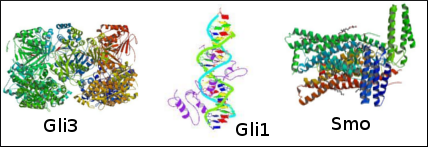
\includegraphics[width=0.8\textwidth]{gli_gli3_smo}
 	\centering
 	\caption{Representación esquemática de la proteinas Gli1, Gli3 y Smo. Fuente: \cite{phosphosite}}
 	\label{figuras}
 \end{figure}
 
 
 
 
 Presentamos el proceso de forma esquemática siguiendo las  indicaciones de \cite{schaffer}:
 \begin{enumerate}
 	\item El \textit{Shh} interactúa con un receptor de superficie celular denominado \textit{Patched }(\textit{Ptc}).
 	\item El \textit{Ptc} inhibe la actividad de señalización de una segunda proteína de la superficie celular: \textit{Smoothened }(\textit{Smo}).
 	\item La unión de \textit{Shh} y \textit{Ptc} neutraliza el efecto inhibidor  de \textit{Ptc} sobre \textit{Smo}.
 	\item Cuando \textit{Smo} no está inhibido afecta a la actividad de la familia de factores de transcripcion \textit{Gli}
 	\item En ausencia de\textit{ Shh, Gli3} es transformado mediante la proteolisis en \textit{Gli3R} (represor de la transcripción génica)
 	\item Tras la señalización de \textit{Shh} y \textit{Smo}, la proteolisis se bloquea, lo que lleva a la acumulación de \textit{Gli3}
 	\item El \textit{Gli3} (activador de la transcripcion génica) activa la transcripcion de los genes \textit{gli1, gli2, ptc, shh.}
 	\item La activación de la transcripción de estos genes provoca la creacion de\textit{ Gli y Ptc}, lo cual a su vez, favorece la generación de \textit{Gli y Ptc}.
 \end{enumerate}
 
 El valor añadido de incluir la ARN polimerasa en el modelo vendrá explicado en la seccion \ref{ch:modelo_alternativo} .
 En la figura \ref{signal_path} se puede encontrar un dibujo esquemático del proceso.
  \begin{figure}[h]
  	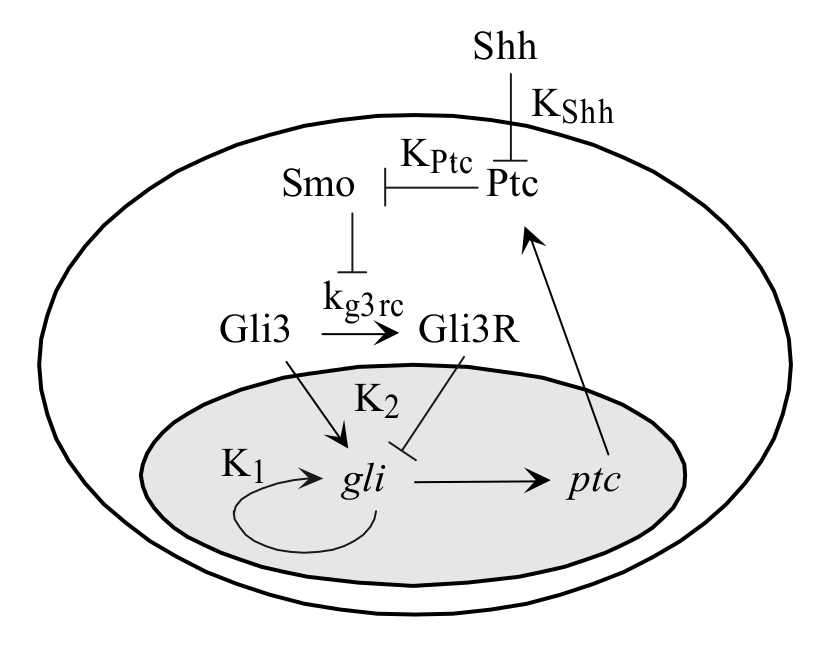
\includegraphics[width=0.8\textwidth]{signal_path}
  	\centering
  	\caption{Representación esquemática de la red de transcripciónn. Fuente: \cite{schaffer}}
  	\label{signal_path}
  \end{figure}
  
 
 
 \subsection{Interacción entre Ptc y Shh}
 Shh y Ptc se unen de forma reversible con una constante de disociación $K_-$ y de asociacion $K_+$. Al cociente entre ambas es lo que denominaremos $K_{Shh}$, mediante el siguiente esquema: 
 
\begin{equation}
\ce{[Shh] + [Ptc] <->[K_{Shh}] [Shh.Ptc] }
\label{s:1}
\end{equation}
 
 Además, asumimos que las uniones entre Ptc y Shh llegan rapidamente a un estado estacionario si tomamos la escala temporal de transcripcion genetica y sisntesis de proteinas. Para conocer cual es, utilizamos la ecuación de Scatchard.
 
 La ecuación de Scatchard es una ecuación utilizada en bioquímica y biología molecular para calcular la constante de afinidad de un ligando con una proteína, propuesta por primera ver en \cite{scatchard1949attractions}. 
 
 Sea una reaccion como (\ref{s:1}) tenemos que: 
 $$K_{Shh}=\frac{[Shh.Ptc]}{[Shh][Ptc]}$$
 de donde 
 $$[Shh.Ptc]=K_{Shh}[Shh][Ptc]$$
 Sea ahora $\nu$ representando los moles de ligando unido por mol de proteina, en primer lugar tenemos:
 \begin{equation}
 \nu=\frac{[Shh.Ptc]}{[Ptc_{Total}]}
 \label{s:2}
 \end{equation}
 
 Ahora bien, si operamos:
 $$\nu=\frac{[Shh.Ptc]}{[Ptc_{Total}]}=\frac{[Shh.Ptc]}{[Ptc.Shh]+[Ptc]}=\frac{K_{Shh}[Shh][Ptc]}{[Ptc]+K_{Shh}[Shh][Ptc]}=\frac{K_{Shh}[Shh]}{1+K_{Shh}[Shh]}$$
 Finalmente:
 \begin{equation}
 \nu=\frac{[Shh]}{[Shh]+K_{Shh}^{-1}}
 \label{s:3}
 \end{equation}
 
 En este caso, uniendo \ref{s:3} y \ref{s:2} expresión: 
 \begin{equation}
 [Shh.Ptc]=\frac{[Shh][Ptc_{Total}]}{K_{Shh}^{-1}+[Shh]}
 \label{s:6}
 \end{equation}
 
 Si bien este es el procedimiento empleado en \cite{schaffer},hacemos notar que las primera relación de Scatchard introducida se puede obtener basándonos en el estado de equilibrio de la ley de acción de masas.
 
 Partiendo asi de \ref{s:1}: 
  \begin{equation}
  \frac{d}{dt}[Shh.Ptc]=k_+[Shh][Ptc]-K^-[Shh.Ptc]
  \label{s:8}
  \end{equation}
 Si suponemos que el compuesto esta en equilibrio:
  \begin{equation}
 \frac{d}{dt}[Shh.Ptc]=0=K_+[Shh][Ptc]-K^-[Shh.Ptc] \implies \frac{[Shh.Ptc]}{[Shh][Ptc]}=K_+/K_- \implies_{def} K_{Shh}
 \label{s:9}
 \end{equation}
 
 Para evitar complicaciones excesivas en la notación, denominaremos a $K_{Shh}^{-1}$ como $k_{Shh}$.
 
 \subsection{Señal de transcripcion}
 Vamos a considerar el término \textbf{\textit{Señal}} como la fracción de \textit{Smo} liberada de la inhibicion del \textit{Ptc}. Aunque Ptc y Smo no interactúan físicamente \cite{schaffer} propone modelarlo de manera similar a la union de Shh y Ptc, puesto que la cantidad de Smo libre puede interpretarse como la cantidad que no esta interactuando de forma eficiente con el Ptc.
 En este caso, tenemos:
 \begin{equation}
 [Shh.Ptc]=\frac{[Ptc_{libre}][Smo_{Total}]}{k_{Ptc}+[Ptc_{libre}]}
 \label{s:5}
 \end{equation}
 Donde $Ptc_{libre}$ hace referencia al Ptc que no está interactuando con Shh y $k_{Ptc}$ es la mitad de la concentración de Ptc necesaria para inhibir la actividad de Smo.
 Tal y como comentamos, definimos la \textbf{\textit{señal}} (en adelante \textit{Signal}) como:
 \begin{equation}
 Signal=\frac{[Smo_{libre}]}{[Smo_{Total}]}=\frac{[Smo_{total}]-[Smo.Ptc]}{[Smo_{Total}]}
 \label{s:4}
 \end{equation}
 Finalmente, usando \ref{s:5} y \ref{s:6} en \ref{s:4} nos queda:
 \begin{equation}
 Signal=\frac{[Smo_{libre}]}{[Smo_{Total}]}=\frac{\frac{Shh}{k_{shh}} + 1}{\frac{Shh}{k_{shh}} + 1 + \frac{Ptc}{k_{ptc}}}
 \label{s:7}
 \end{equation}
 
 \subsection{Dinámica de Gli3 y Gli3R}
 \subsubsection{Dinámica de Gli3}
 En ausencia de señalización Shh, Gli3 se escinde proteolíticamente en un fragmento que funciona como un
 represor transcripcional.En \cite{wang2000hedgehog} muestran que el grado de proteólisis disminuye con el aumento de Shh. En este caso, imponemos que la tasa de proteólisis varíe inversamente con el nivel de señalización Shh en el sistema.
 
 Así, nuestra la cantidad de Gli3 disminuye con una tasa $k_{g3rc}$ que se modifica por la cantidad de $Signal$ en el sistema y un parámetro de saturación $K_g3rc$.
 
 A su vez, se ha demostrado que a medida que se activa la red de regulación génica, gli3 es transcripcionalmente
 reprimido \cite{wang2000hedgehog}. Dos lecturas del grado de activación de nuestra red son Ptc y Gli. 
 
 \textbf{\textit{Esto es importante, puesto que, aunque Ptc ofrece tambien una lectura del grado de activación, los resultados pueden variar en gran cantidad dependiendo de cual elijamos.}}
 
 Por lo tanto, asumimos una relación inversa entre la transcripcion de gli3 y la concentración de Gli en las ecuaciones para Gli3, partiendo de una tasa basal de generacion de Gli3 que viene dada por la constante $r_{g3b}$. 
 
 Finalmente, con toda la información podemos entender como modelar matemáticamente la evolución de Gli3:
 
  \begin{equation}
  \frac{dGli_3}{dt} = \frac{r_{g3b}}{Gli}-k_{deg}Gli_3-\left(\frac{k_{g3rc}}{K_{g3rc}+Signal}\right)Gli_3,
  \end{equation}
 
 \subsubsection{Dinámica de Gli3R}
 La existencia de esta molecula es completamente dependiente a la existencia de Gli3.
 
 En su dinámica vamos a encontrar un término positivo exactamente igual a la rapidez en la que Gli3 es separado de forma proteolitica y, además, un término de degradacion (cuya constate de degradación es igual a la constante de degradación de Gli3).
 
  Esto nos deja con la expresión:

 
 \begin{equation}
 \frac{dGli3R}{dt}= \left(\frac{k_{g3rc}}{K_{g3rc}+Signal}\right)Gli_3-k_{deg}Gli3R,
 \end{equation}
 
 \section{Modelado BEWARE}
 
 \subsubsection{Enfoques en el modelado de la regulación génica}
 
 El análisis detallado de las redes transcripcionales es clave para comprender los procesos biológicos centrales. Modelar correctamente la regulación de genes es fundamental para tal fin, puesto que la expresión génica está en el nexo de muchos procesos biológicos, y los cambios en los niveles de proteínas reguladoras o enlaces pueden ser la base de, por ejemplo, enfermedades de gran impacto como el cáncer. 
 
  A la hora de profundizar y aportar nuevo conocimiento en este área,las matemáticas se han desarrollado por diversos caminos, resaltando unas u otras características. Como se destaca en \cite{ay2011mathematical} dentro de este actual abanico de técnicas tenemos dos grandes estrategias iniciales: \textit{Enfoque analítico o estadístico}. 
  
  Durante nuestro trabajo nos hemos centrado en el primero. Dentro del cual podemos encontrar tres grandes ramas: \textit{modelos termodinámicos, booleanos y de ecuaciones diferenciales}. Cada una de los cuales debe ser tomada con cautela para obtener el máximo beneficio en cuanto al conocimiento del comportamiento cualitativo y cuantitativo de las soluciones. 
 
 Lo más habitual presentado en el grado y en el máster son los modelos basados en ecuaciones diferenciales, ya sean ordinarias o en derivadas parciales. Estos modelos surgen de la necesidad de crear sistemas dinámicos con muchas componentes que evoluciones a lo largo del tiempo. Como hemos visto en la sección anterior, esta técnica ha sido empleada por los dos modelos estudiados, en aquellos comportamientos dependientes de proteínas que modelaban la asociación y disociación de compuestos.
 
 Sin embargo, a la hora de modelar el proceso de transcripción genética, tanto para \textit{Gli} como para \textit{Ptc}, el modelado va a seguir \textbf{el enfoque termodinámico}. 
 
 Antes de continuar vamos a ofrecer una breve descripción generalista del proceso general que planteamos modelar: la transcripción génica.
 
 \subsubsection{Biología de la transcripción génica}
 Segun se expone en \cite{biologia}, el proceso general de transcripción es un proceso biológico complejo. En primer lugar la enzima ARN polimerasa (ARNp), que forma una nueva molécula de ARN a partir del código proporcionado por el ADN, debe unirse al ADN del gen. Se adjunta en un lugar anterior al código genético que queremos transcribir. Esta zona se conoce como \textbf{promotor}.
 
 La \textbf{ARNp} necesita de ayuda para unirse a esta sección. COn este fin aparecen conjunto de proteínas llamadas factores de transcripción.\footnote{Hay muchos tipos de factores de transcripción. Aunque su función en ocasiones puede ser desempeñada por factores de transcripcion generales, existe una gran clase de factores de transcripción que controlan la expresión de genes individuales específicos.}
 
 Vamos a detenernos en esta parte, para comprender mejor los factores de transcripción, puesto que juegan un papel importante en el modelado.
  Un factor de transcripción típico se une al ADN en una determinada secuencia diana \footnote{Los sitios de unión para los factores de transcripción a menudo están cerca del promotor de un gen. Sin embargo, se pueden encontrar en otras partes del ADN, a veces muy lejos del promotor, y aún afectan la transcripción del gen.}. Una vez que está unido, el factor de transcripción hace que sea más difícil o más fácil que la ARN polimerasa se una al promotor del gen. Con esto en mente, podemos clasificar este tipo de factores de activación, según faciliten o dificulten esta unión.
 
 Por un lado algunos factores de transcripción activan la transcripción. Por ejemplo, pueden ayudar a que los factores de transcripción generales y / o la ARN polimerasa se unan al promotor.
 
 Otros factores de transcripción reprimen la transcripción. Esta represión puede funcionar en una variedad de formas. Como un ejemplo, un represor puede interferir con los factores de transcripción basales o la ARN polimerasa, por lo que no pueden unirse al promotor o comenzar la transcripción.
 
 Además, hay otro actor reseñable dentro de este procedimiento. Los potenciadores son una secuencia de ADN que puede activar el uso de un promotor, controlando la eficiencia y la tasa de transcripción de ese promotor particular.
 
 En general, estos son los factores a tener en cuenta en la transcripxion genica. A modo de resumen dejamos la grafica \ref{biologiafoto} y \ref{biofoto2}.
   \begin{figure}[h]
 	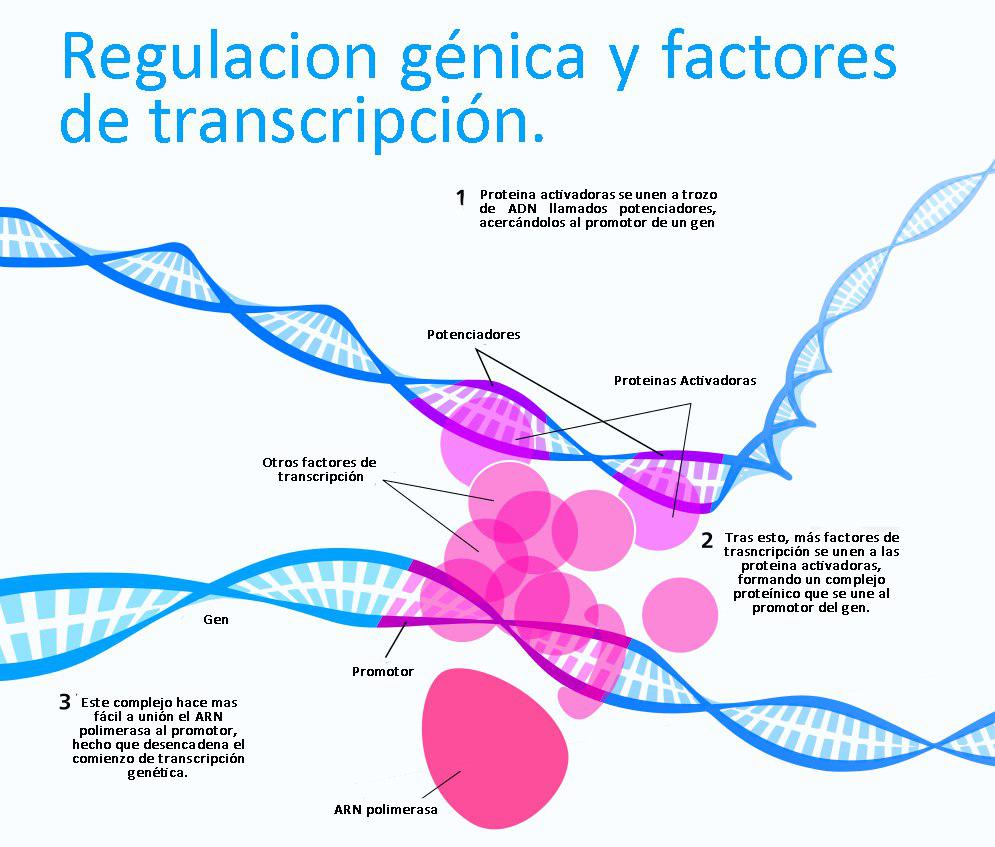
\includegraphics[width=1\textwidth]{fotobio}
 	\centering
 	\caption{Representación artística de la transcripción génica}
 	\label{biologiafoto}
 \end{figure}
    \begin{figure}[h]
 	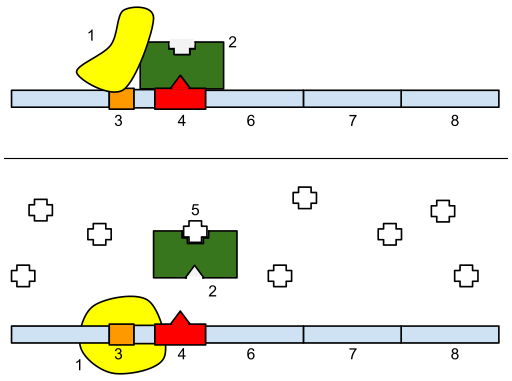
\includegraphics[width=0.8\textwidth]{fotobio2}
 	\centering
 	\caption{\textbf{1: ARN polimerasa, 2: represor, 3: promotor, 4: operador, 5: lactosa, 6-8: Genes.} Arriba: el gen está esencialmente desactivado. Abajo: el gen está encendido}
 	\label{biofoto2}
 \end{figure}
 
 \subsubsection{Modelado termodinámico}
 
 Este enfoque de modelado, como apunta \cite{ay2011mathematical}, busca extraer información sobre la regulación génica a partir de las secuencias de las regiones reguladoras y la unión medida o inferida de los factores de transcripción específicos.
 
 Es decir, supongamos que tenemos un promotor y algunos factores de transcripción que reprimen o promueven esta transcripción. En este caso, nuestro modelado quiere predecir cómo se activará o reprimirá la transcripccion de un gen según estos factores y sus cantidades.
 
 
 La clave fundamental modelando termodinámicamente es el calculo de cómo las diferentes combinaciones de distintos lugares y números de unión en una región reguladora funcionan juntos para producir la expresión a lo largo del tiempo de un gen.
 
 A grandes rasgos suponemos que la actividad del gen es proporcional al nivel de activadores unidos e inversamente proporcional al nivel de represores.
 
 \subsubsection{Procedimiento}
 
  Sea cual sea la estrategia a seguir, modelado termodinámico sigue dos pasos comunes a todos los modelos de esta rama:
  \begin{itemize}
  	\item En primer lugar: se enumeran todos los estados posibles del potenciador, en función de las posibles interacciones entre el factor de transcripción y el ADN, con un peso estadístico asignado a cada estado.
  	\item  El segundo lugar calculamos el resultado de la expresión génica de cada estado. Los estados con alta ocupación de activadores son más proclives a inducir una expresión alta, mientras que la ocupación del represor puede dar como resultado una baja expresión.
  \end{itemize}
  
   Durante el primer paso es indispensable el calculo de la probabilidad de que un gen se ponga en funcionamiento, para ello calculamos la fracción de los estados con una cantidad de activadores unidos destacable frente a represores.
   
   Esto por si solo ya genera una gran cantidad de estados a tener en cuenta, pensemos en nuestro caso: nuestra región regulatoria tiene tres lugares de unión, por tanto habrá nueve estados posibles, vinculados y no vinculados. Si queremos añadir nueva información (por ejemplo si nos interesamos por elementos con ccinco lugares de unión) el numero de estados aumenta considerablemente (en nuestro caso hipotético 25 entre vinculados y no vinculados).
 
 
 Otro de los factores a tener en cuenta es el calculo del peso estadístico para un estado. Para ello usamos la concentración de factores de transcripción
 y la afinidad de estos factores por sus sitios en el ADN. Para una unión abundante de proteínas a sitios de alta afinidad, el peso será mucho mayor que en los casos en que la transcripción el factor es escaso o el sitio de unión es débil.
  La probabilidad de cada estado se puede calcular por
 dividiendo el peso estadístico del estado por la suma del peso estadístico de todos los posibles
 estados. 
 
 
 Este proceso de cálculo puede incorporar propiedades que afectan la transcripción. por ejemplo, interacciones cooperativas y competitivas entre factores de transcripción y los efectos inhibidores de los represores sobre los activadores se pueden agregar explícitamente al modelo asignando pesos más altos o más bajos.
 
 Como podemos observar, estamos ante una forma de modelado que nos da bastante juego a la hora de modificar distintos parámetros y procedimientos. En particular, vamos a resaltar la mayor diferencia entre los distintos modelados que se han empleado en este trabajo:
 \begin{itemize}
 	\item \cite{schaffer} modela la expresión génica como cantidad proporcional a la suma ponderada de los factores de transcripción(\textit{ enfoque stimulated}).
 	\item Por otra parte, \cite{cambon1} proponen que la expresión génica sea proporcional a la probabilidad de unión del ARN-polimerasa (\textit{ enfoque recruitment}), la cual viene modificada por los factores de transcripción.
 		
 		
 	\end{itemize}
 
 
 
 
 \subsubsection{Críticas recibidas}
 
 
 Finalmente, como último apunte, aunque partimos un de una forma de modelado con amplios resultados queremos resaltar algunas de las criticas que ha recibido esta forma de modelar.
 
 La implementación actual ignora procesos adicionales como la estructura y modificación de la cromatina, o la metilación del ADN, y no trata de forma independiente el reclutamiento de cofactores o la maquinaria general de transcripción.
 
  Se entiende actualmente que estos saltos teoricos no aportan gran información al sistema tal y como se expone en \cite{ay2011mathematical}, aún así, creemos que es conveniente no perderlos de vista, debido a que es un cambio en los objetivos de los que se pretende modelar (nuestro nuevo modelo incluye la actividad de la ARN polimerasa) lo que ha supuesto un esperanzador cambio en el ajuste de este modelo con la realidad.